
%% bare_jrnl_compsoc.tex
%% V1.4b
%% 2015/08/26
%% by Michael Shell
%% See:
%% http://www.michaelshell.org/
%% for current contact information.
%%
%% This is a skeleton file demonstrating the use of IEEEtran.cls
%% (requires IEEEtran.cls version 1.8b or later) with an IEEE
%% Computer Society journal paper.
%%
%% Support sites:
%% http://www.michaelshell.org/tex/ieeetran/
%% http://www.ctan.org/pkg/ieeetran
%% and
%% http://www.ieee.org/

%%*************************************************************************
%% Legal Notice:
%% This code is offered as-is without any warranty either expressed or
%% implied; without even the implied warranty of MERCHANTABILITY or
%% FITNESS FOR A PARTICULAR PURPOSE!
%% User assumes all risk.
%% In no event shall the IEEE or any contributor to this code be liable for
%% any damages or losses, including, but not limited to, incidental,
%% consequential, or any other damages, resulting from the use or misuse
%% of any information contained here.
%%
%% All comments are the opinions of their respective authors and are not
%% necessarily endorsed by the IEEE.
%%
%% This work is distributed under the LaTeX Project Public License (LPPL)
%% ( http://www.latex-project.org/ ) version 1.3, and may be freely used,
%% distributed and modified. A copy of the LPPL, version 1.3, is included
%% in the base LaTeX documentation of all distributions of LaTeX released
%% 2003/12/01 or later.
%% Retain all contribution notices and credits.
%% ** Modified files should be clearly indicated as such, including  **
%% ** renaming them and changing author support contact information. **
%%*************************************************************************


% *** Authors should verify (and, if needed, correct) their LaTeX system  ***
% *** with the testflow diagnostic prior to trusting their LaTeX platform ***
% *** with production work. The IEEE's font choices and paper sizes can   ***
% *** trigger bugs that do not appear when using other class files.       ***                          ***
% The testflow support page is at:
% http://www.michaelshell.org/tex/testflow/


\documentclass[10pt,journal,compsoc]{IEEEtran}
%
% If IEEEtran.cls has not been installed into the LaTeX system files,
% manually specify the path to it like:
% \documentclass[10pt,journal,compsoc]{../sty/IEEEtran}





% Some very useful LaTeX packages include:
% (uncomment the ones you want to load)


% *** MISC UTILITY PACKAGES ***
%
%\usepackage{ifpdf}
% Heiko Oberdiek's ifpdf.sty is very useful if you need conditional
% compilation based on whether the output is pdf or dvi.
% usage:
% \ifpdf
%   % pdf code
% \else
%   % dvi code
% \fi
% The latest version of ifpdf.sty can be obtained from:
% http://www.ctan.org/pkg/ifpdf
% Also, note that IEEEtran.cls V1.7 and later provides a builtin
% \ifCLASSINFOpdf conditional that works the same way.
% When switching from latex to pdflatex and vice-versa, the compiler may
% have to be run twice to clear warning/error messages.






% *** CITATION PACKAGES ***
%
\ifCLASSOPTIONcompsoc
  % IEEE Computer Society needs nocompress option
  % requires cite.sty v4.0 or later (November 2003)
  \usepackage[nocompress]{cite}
\else
  % normal IEEE
  \usepackage{cite}
\fi
% cite.sty was written by Donald Arseneau
% V1.6 and later of IEEEtran pre-defines the format of the cite.sty package
% \cite{} output to follow that of the IEEE. Loading the cite package will
% result in citation numbers being automatically sorted and properly
% "compressed/ranged". e.g., [1], [9], [2], [7], [5], [6] without using
% cite.sty will become [1], [2], [5]--[7], [9] using cite.sty. cite.sty's
% \cite will automatically add leading space, if needed. Use cite.sty's
% noadjust option (cite.sty V3.8 and later) if you want to turn this off
% such as if a citation ever needs to be enclosed in parenthesis.
% cite.sty is already installed on most LaTeX systems. Be sure and use
% version 5.0 (2009-03-20) and later if using hyperref.sty.
% The latest version can be obtained at:
% http://www.ctan.org/pkg/cite
% The documentation is contained in the cite.sty file itself.
%
% Note that some packages require special options to format as the Computer
% Society requires. In particular, Computer Society  papers do not use
% compressed citation ranges as is done in typical IEEE papers
% (e.g., [1]-[4]). Instead, they list every citation separately in order
% (e.g., [1], [2], [3], [4]). To get the latter we need to load the cite
% package with the nocompress option which is supported by cite.sty v4.0
% and later. Note also the use of a CLASSOPTION conditional provided by
% IEEEtran.cls V1.7 and later.





% *** GRAPHICS RELATED PACKAGES ***
%
\ifCLASSINFOpdf
  % \usepackage[pdftex]{graphicx}
  % declare the path(s) where your graphic files are
  % \graphicspath{{../pdf/}{../jpeg/}}
  % and their extensions so you won't have to specify these with
  % every instance of \includegraphics
  % \DeclareGraphicsExtensions{.pdf,.jpeg,.png}
\else
  % or other class option (dvipsone, dvipdf, if not using dvips). graphicx
  % will default to the driver specified in the system graphics.cfg if no
  % driver is specified.
  % \usepackage[dvips]{graphicx}
  % declare the path(s) where your graphic files are
  % \graphicspath{{../eps/}}
  % and their extensions so you won't have to specify these with
  % every instance of \includegraphics
  % \DeclareGraphicsExtensions{.eps}
\fi
% graphicx was written by David Carlisle and Sebastian Rahtz. It is
% required if you want graphics, photos, etc. graphicx.sty is already
% installed on most LaTeX systems. The latest version and documentation
% can be obtained at:
% http://www.ctan.org/pkg/graphicx
% Another good source of documentation is "Using Imported Graphics in
% LaTeX2e" by Keith Reckdahl which can be found at:
% http://www.ctan.org/pkg/epslatex
%
% latex, and pdflatex in dvi mode, support graphics in encapsulated
% postscript (.eps) format. pdflatex in pdf mode supports graphics
% in .pdf, .jpeg, .png and .mps (metapost) formats. Users should ensure
% that all non-photo figures use a vector format (.eps, .pdf, .mps) and
% not a bitmapped formats (.jpeg, .png). The IEEE frowns on bitmapped formats
% which can result in "jaggedy"/blurry rendering of lines and letters as
% well as large increases in file sizes.
%
% You can find documentation about the pdfTeX application at:
% http://www.tug.org/applications/pdftex






% *** MATH PACKAGES ***
%
%\usepackage{amsmath}
% A popular package from the American Mathematical Society that provides
% many useful and powerful commands for dealing with mathematics.
%
% Note that the amsmath package sets \interdisplaylinepenalty to 10000
% thus preventing page breaks from occurring within multiline equations. Use:
%\interdisplaylinepenalty=2500
% after loading amsmath to restore such page breaks as IEEEtran.cls normally
% does. amsmath.sty is already installed on most LaTeX systems. The latest
% version and documentation can be obtained at:
% http://www.ctan.org/pkg/amsmath





% *** SPECIALIZED LIST PACKAGES ***
%
%\usepackage{algorithmic}
% algorithmic.sty was written by Peter Williams and Rogerio Brito.
% This package provides an algorithmic environment fo describing algorithms.
% You can use the algorithmic environment in-text or within a figure
% environment to provide for a floating algorithm. Do NOT use the algorithm
% floating environment provided by algorithm.sty (by the same authors) or
% algorithm2e.sty (by Christophe Fiorio) as the IEEE does not use dedicated
% algorithm float types and packages that provide these will not provide
% correct IEEE style captions. The latest version and documentation of
% algorithmic.sty can be obtained at:
% http://www.ctan.org/pkg/algorithms
% Also of interest may be the (relatively newer and more customizable)
% algorithmicx.sty package by Szasz Janos:
% http://www.ctan.org/pkg/algorithmicx




% *** ALIGNMENT PACKAGES ***
%
%\usepackage{array}
% Frank Mittelbach's and David Carlisle's array.sty patches and improves
% the standard LaTeX2e array and tabular environments to provide better
% appearance and additional user controls. As the default LaTeX2e table
% generation code is lacking to the point of almost being broken with
% respect to the quality of the end results, all users are strongly
% advised to use an enhanced (at the very least that provided by array.sty)
% set of table tools. array.sty is already installed on most systems. The
% latest version and documentation can be obtained at:
% http://www.ctan.org/pkg/array


% IEEEtran contains the IEEEeqnarray family of commands that can be used to
% generate multiline equations as well as matrices, tables, etc., of high
% quality.




% *** SUBFIGURE PACKAGES ***
%\ifCLASSOPTIONcompsoc
%  \usepackage[caption=false,font=footnotesize,labelfont=sf,textfont=sf]{subfig}
%\else
%  \usepackage[caption=false,font=footnotesize]{subfig}
%\fi
% subfig.sty, written by Steven Douglas Cochran, is the modern replacement
% for subfigure.sty, the latter of which is no longer maintained and is
% incompatible with some LaTeX packages including fixltx2e. However,
% subfig.sty requires and automatically loads Axel Sommerfeldt's caption.sty
% which will override IEEEtran.cls' handling of captions and this will result
% in non-IEEE style figure/table captions. To prevent this problem, be sure
% and invoke subfig.sty's "caption=false" package option (available since
% subfig.sty version 1.3, 2005/06/28) as this is will preserve IEEEtran.cls
% handling of captions.
% Note that the Computer Society format requires a sans serif font rather
% than the serif font used in traditional IEEE formatting and thus the need
% to invoke different subfig.sty package options depending on whether
% compsoc mode has been enabled.
%
% The latest version and documentation of subfig.sty can be obtained at:
% http://www.ctan.org/pkg/subfig




% *** FLOAT PACKAGES ***
%
%\usepackage{fixltx2e}
% fixltx2e, the successor to the earlier fix2col.sty, was written by
% Frank Mittelbach and David Carlisle. This package corrects a few problems
% in the LaTeX2e kernel, the most notable of which is that in current
% LaTeX2e releases, the ordering of single and double column floats is not
% guaranteed to be preserved. Thus, an unpatched LaTeX2e can allow a
% single column figure to be placed prior to an earlier double column
% figure.
% Be aware that LaTeX2e kernels dated 2015 and later have fixltx2e.sty's
% corrections already built into the system in which case a warning will
% be issued if an attempt is made to load fixltx2e.sty as it is no longer
% needed.
% The latest version and documentation can be found at:
% http://www.ctan.org/pkg/fixltx2e


%\usepackage{stfloats}
% stfloats.sty was written by Sigitas Tolusis. This package gives LaTeX2e
% the ability to do double column floats at the bottom of the page as well
% as the top. (e.g., "\begin{figure*}[!b]" is not normally possible in
% LaTeX2e). It also provides a command:
%\fnbelowfloat
% to enable the placement of footnotes below bottom floats (the standard
% LaTeX2e kernel puts them above bottom floats). This is an invasive package
% which rewrites many portions of the LaTeX2e float routines. It may not work
% with other packages that modify the LaTeX2e float routines. The latest
% version and documentation can be obtained at:
% http://www.ctan.org/pkg/stfloats
% Do not use the stfloats baselinefloat ability as the IEEE does not allow
% \baselineskip to stretch. Authors submitting work to the IEEE should note
% that the IEEE rarely uses double column equations and that authors should try
% to avoid such use. Do not be tempted to use the cuted.sty or midfloat.sty
% packages (also by Sigitas Tolusis) as the IEEE does not format its papers in
% such ways.
% Do not attempt to use stfloats with fixltx2e as they are incompatible.
% Instead, use Morten Hogholm'a dblfloatfix which combines the features
% of both fixltx2e and stfloats:
%
% \usepackage{dblfloatfix}
% The latest version can be found at:
% http://www.ctan.org/pkg/dblfloatfix




%\ifCLASSOPTIONcaptionsoff
%  \usepackage[nomarkers]{endfloat}
% \let\MYoriglatexcaption\caption
% \renewcommand{\caption}[2][\relax]{\MYoriglatexcaption[#2]{#2}}
%\fi
% endfloat.sty was written by James Darrell McCauley, Jeff Goldberg and
% Axel Sommerfeldt. This package may be useful when used in conjunction with
% IEEEtran.cls'  captionsoff option. Some IEEE journals/societies require that
% submissions have lists of figures/tables at the end of the paper and that
% figures/tables without any captions are placed on a page by themselves at
% the end of the document. If needed, the draftcls IEEEtran class option or
% \CLASSINPUTbaselinestretch interface can be used to increase the line
% spacing as well. Be sure and use the nomarkers option of endfloat to
% prevent endfloat from "marking" where the figures would have been placed
% in the text. The two hack lines of code above are a slight modification of
% that suggested by in the endfloat docs (section 8.4.1) to ensure that
% the full captions always appear in the list of figures/tables - even if
% the user used the short optional argument of \caption[]{}.
% IEEE papers do not typically make use of \caption[]'s optional argument,
% so this should not be an issue. A similar trick can be used to disable
% captions of packages such as subfig.sty that lack options to turn off
% the subcaptions:
% For subfig.sty:
% \let\MYorigsubfloat\subfloat
% \renewcommand{\subfloat}[2][\relax]{\MYorigsubfloat[]{#2}}
% However, the above trick will not work if both optional arguments of
% the \subfloat command are used. Furthermore, there needs to be a
% description of each subfigure *somewhere* and endfloat does not add
% subfigure captions to its list of figures. Thus, the best approach is to
% avoid the use of subfigure captions (many IEEE journals avoid them anyway)
% and instead reference/explain all the subfigures within the main caption.
% The latest version of endfloat.sty and its documentation can obtained at:
% http://www.ctan.org/pkg/endfloat
%
% The IEEEtran \ifCLASSOPTIONcaptionsoff conditional can also be used
% later in the document, say, to conditionally put the References on a
% page by themselves.




% *** PDF, URL AND HYPERLINK PACKAGES ***
%
%\usepackage{url}
% url.sty was written by Donald Arseneau. It provides better support for
% handling and breaking URLs. url.sty is already installed on most LaTeX
% systems. The latest version and documentation can be obtained at:
% http://www.ctan.org/pkg/url
% Basically, \url{my_url_here}.





% *** Do not adjust lengths that control margins, column widths, etc. ***
% *** Do not use packages that alter fonts (such as pslatex).         ***
% There should be no need to do such things with IEEEtran.cls V1.6 and later.
% (Unless specifically asked to do so by the journal or conference you plan
% to submit to, of course. )
\usepackage{cite}
\usepackage{amsmath,amssymb,amsfonts}
\usepackage{algorithmic}
\usepackage{graphicx}
\usepackage{textcomp}
\usepackage[svgnames]{xcolor}
\usepackage{latexsym}
\usepackage{amsfonts}
\usepackage{amsmath}
\usepackage{amssymb}
\usepackage{color}
\usepackage{epsfig}
\usepackage{xspace}
\usepackage{graphicx}
\usepackage{subfigure}
\usepackage{balance}
\usepackage{rotating}
\usepackage{pbox}
\usepackage{caption}
\usepackage{epsfig}
\usepackage{multirow}
\usepackage{url}
\usepackage[implicit=false]{hyperref}
%%%%%%%%%%%%%%%%%%%%%%%%%%
%%%%%%%%%New added packages
%%%%%%%%%%%%%%%%%%%%%%%%%
\usepackage{mathrsfs}

\newcommand{\imp}{\vdash_{\cal I}}

%%%%%%%%%%%%%%%%%%%%%%%%%%%%%%%%%%%%%%%%%%
% Enumerate and Itemize modifications
\usepackage{enumitem}
\setlist{topsep=0pt,noitemsep} \setitemize[1]{label=$\circ$}
%%%%%%%%%%%%%%%%%%%%%%%%%%%%%%%%%%%%%%%%%%%

\sloppy
\newcommand{\rtable}[1]{\ensuremath{\mathsf{#1}}}
\newcommand{\ratt}[1]{\ensuremath{\mathit{#1}}}
\newcommand{\at}[1]{\protect\ensuremath{\mathsf{#1}}\xspace}
\newcommand{\myhrule}{\rule[.5pt]{\hsize}{.5pt}}
\newcommand{\oneurl}[1]{\texttt{#1}}
\newcommand{\eat}[1]{}
\newcommand{\stab}{\rule{0pt}{8pt}\\[-1.6ex]}
\newcommand{\sttab}{\rule{0pt}{8pt}\\[-2ex]}
\newcommand{\sstab}{\rule{0pt}{8pt}\\[-2.4ex]}
\newcommand{\tabstrut}{\rule{0pt}{4pt}\vspace{-0.07in}}
\newcommand{\vs}{\vspace{1ex}}
\newcommand{\exa}[2]{{\tt\begin{tabbing}\hspace{#1}\=\+\kill #2\end{tabbing}}}
\newcommand{\ra}{\rightarrow}
\newcommand{\la}{\leftarrow}
\newcommand{\bi}{\begin{itemize}}
\newcommand{\ei}{\end{itemize}}
\newenvironment{tbi}{\begin{itemize}
        \setlength{\topsep}{1.5ex}\setlength{\itemsep}{0ex}}
%\vspace{-0.5ex}}
        {\end{itemize}\vspace{-0.5ex}}
\newenvironment{tbe}{\begin{enumerate}
        \setlength{\topsep}{0ex}\setlength{\itemsep}{0ex}\vspace{0ex}}
        {\end{itemize}\vspace{-1ex}}

\newcommand{\noteqs}[1]{{\color{red}{#1}---QS}}

\newcommand{\mat}[2]{{\begin{tabbing}\hspace{#1}\=\+\kill #2\end{tabbing}}}
\newcommand{\m}{\hspace{0.05in}}
\newcommand{\ls}{\hspace{0.1in}}
\newcommand{\be}{\begin{enumerate}}
\newcommand{\ee}{\end{enumerate}}
\newcommand{\beqn}{\begin{eqnarray*}}
\newcommand{\eeqn}{\end{eqnarray*}}
\newcommand{\card}[1]{\mid\! #1\!\mid}
\newcommand{\fth}{\hfill $\Box$}
\newcommand{\AND}{\displaystyle{\bigwedge_{i=1}^{n}}}
\newcommand{\U}[1]{\displaystyle{\bigcup_{#1}}}
\newcommand{\Sm}[1]{\displaystyle{\sum_{#1}}}
\newcommand{\stitle}[1]{\vspace{1.5ex}\noindent{\bf #1}}
\newcommand{\etitle}[1]{\vspace{0.8ex}\noindent{\em #1}}
\renewcommand{\t}{\tau}
\newcommand{\Inh}[1]{\$#1}
\renewcommand{\r}[1]{{\it rule}(#1)}
\newcommand{\pa}{\parallel}
\newcommand{\LHS}{\kw{{\small LHS}}\xspace}
\newcommand{\RHS}{\kw{RHS}\xspace}
\newcommand{\ie}{\emph{i.e.,}\xspace}
\newcommand{\eg}{\emph{e.g.,}\xspace}
\newcommand{\wrt}{\emph{w.r.t.}\xspace}
\newcommand{\aka}{\emph{a.k.a.}\xspace}
\newcommand{\kwlog}{\emph{w.l.o.g.}\xspace}
%%%%%%%%%%%%%%%%%%%%%%%%%%%%%%%%%%%%%%%%%%%%%%%%%%%%%%%%%%%%%%%%
%                  Relation Algebra operators
%%%%%%%%%%%%%%%%%%%%%%%%%%%%%%%%%%%%%%%%%%%%%%%%%%%%%%%%%%%%%%%%


\newcommand{\RS}{{\small S}\xspace}
\newcommand{\RP}{{\small P}\xspace}
\newcommand{\RJ}{{\sc j}\xspace}
\newcommand{\RC}{{\small C}\xspace}
\newcommand{\RSJ}{{\small SJ}\xspace}
\newcommand{\RSC}{{\small SC}\xspace}
\newcommand{\RSP}{{\small SP}\xspace}
\newcommand{\RPJ}{{\small PJ}\xspace}
\newcommand{\RPC}{{\small PC}\xspace}
\newcommand{\RSPJ}{{\sc spj}\xspace}
\newcommand{\RSPC}{{\small SPC}\xspace}
\newcommand{\RSPJU}{{\sc spju}\xspace}
\newcommand{\RSPCU}{{\small SPCU}\xspace}
\newcommand{\RSPJUN}{{\small SPJU$^N$}\xspace}
\newcommand{\RSPCUN}{{\small SPCU$^N$}\xspace}

%%%%%%%%%%%%%%%%%%%%%%%%%%%%
% operators
%%%%%%%%%%%%%%%%%%%%%%%%%%%%
\DeclareMathOperator*{\argmin}{arg\,min}

%%%%%%%%%%%%%%%%%%%%%%%%%%%%%%%%%%%%%%%%%%%%%%%%%%%%%%%%%%%%%%%%%%%%%%%%%%%%%%
% ALGORITHMS
%%%%%%%%%%%%%%%%%%%%%%%%%%%%%%%%%%%%%%%%%%%%%%%%%%%%%%%%%%%%%%%%%%%%%%%%%%%%%%%
\newcommand{\SELECT}{\mbox{{\bf select}}\ }
\newcommand{\FROM}{\mbox{{\bf from}\ }}
\newcommand{\WHERE}{\mbox{\bf where}\ }
\newcommand{\SUM}{\mbox{{\bf sum}}\ }
\newcommand{\GROUPBY}{\mbox{{\bf group by}}\ }
\newcommand{\HAVING}{\mbox{{\bf having}}\ }
\newcommand{\CASE}{\mbox{{\bf case}}\ }
\newcommand{\END}{\mbox{{\bf end}}\ }
\newcommand{\WHEN}{\mbox{{\bf when}}\ }
\newcommand{\EXISTS}{\mbox{{\bf exists}}\ }
\newcommand{\COUNT}{\mbox{\kw{count}}}
\newcommand{\INSERTINTO}{\mbox{{\bf insert into}}\ }
\newcommand{\UPDATE}{\mbox{{\bf update}}\ }
\newcommand{\SET}{\mbox{{\bf set}}\ }
\newcommand{\IN}{\mbox{{\bf in}}\ }
\newcommand{\If}{\mbox{\bf if}\ }
\newcommand{\Let}{\mbox{\bf let}\ }
\newcommand{\Call}{\mbox{\bf call}\ }
\newcommand{\Then}{\mbox{\bf then}\ }
\newcommand{\To}{\mbox{\bf to}\ }
\newcommand{\Else}{\mbox{\bf else}\ }
\newcommand{\ElseIf}{\mbox{\bf elseif}\ }
\newcommand{\While}{\mbox{\bf while}\ }
\newcommand{\Begin}{\mbox{\bf begin}\ }
\newcommand{\End}{\mbox{\bf end}\ }
\newcommand{\Do}{\mbox{\bf do}\ }
\newcommand{\Downto}{\mbox{\bf downto}\ }
\newcommand{\Repeat}{\mbox{\bf repeat}\ }
\newcommand{\Until}{\mbox{\bf until}\ }
\newcommand{\For}{\mbox{\bf for}\ }
\newcommand{\Each}{\mbox{\bf each}\ }

\newcommand{\ForEach}{\mbox{\bf for each}\ }
\newcommand{\Or}{\mbox{\bf or}\ }
\renewcommand{\And}{\mbox{\bf and}\ }
\newcommand{\Not}{\mbox{\bf not}\ }
\newcommand{\Break}{\mbox{\bf break}\ }
\newcommand{\Continue}{\mbox{\bf continue}\ }
\newcommand{\Return}{\mbox{\bf return}\ }
\newcommand{\Case}{\mbox{\bf case}\ }
\newcommand{\Of}{\mbox{\bf of}\ }
\newcommand{\EndCase}{\mbox{\bf end-case}\ }
\newcommand{\NIL}{\mbox{\em nil}}
\newcommand{\False}{\mbox{\em false}}
\newcommand{\True}{\mbox{\em true}}
\newcommand{\algAND}{{\sc and}\xspace}
\newcommand{\OR}{{\sc or}\xspace}
\newcommand{\NOT}{{\sc not}\xspace}
\newcommand{\kw}[1]{{\ensuremath {\mathsf{#1}}}\xspace}
\newcommand{\Reps}{S}
\newcounter{ccc}
\newcommand{\bcc}{\setcounter{ccc}{1}\theccc.}
\newcommand{\icc}{\addtocounter{ccc}{1}\theccc.}
\newcommand{\checking}{{\mbox{\small\sf Checking}\xspace}}
\newcommand{\preProcessing}{{\mbox{\small\sf preProcessing}\xspace}}
\newcommand{\CFDconsistency}{{\mbox{\small\sf CFD\_Checking}\xspace}}
\newcommand{\MCS} {\kw{MCS}}
\newcommand{\templateDB}{{\mbox{\small\sf templateDB}\xspace}}
\newcommand{\ChaseChecking}{{\mbox{\small\sf RandomChecking}\xspace}}
\newcommand{\chase}{{\mbox{\small\sf Chase}\xspace}}
\newcommand{\SAT}{{\mbox{\small\sf SAT}\xspace}}
\newcommand{\kSAT}{{\mbox{\small 3SAT}\xspace}}
\newcommand{\PropCFDSPC}{\kw{Prop{\small CFD\_SPC}}}
\newcommand{\PropCFDSPCU}{\kw{Prop{\small CFD\_SPCU}}}
\newcommand{\UnionEQs}{\kw{UnionEQs}}
\newcommand{\UnionCFDs}{\kw{UnionCFDs}}
\newcommand{\EQ}{\kw{EQ}}
\newcommand{\eq}{\kw{eq}}
\newcommand{\key}{\kw{key}}
\newcommand{\rep}{\kw{rep}}
\newcommand{\PEQ}{\kw{EQ2CFD}}
\newcommand{\Drop}{\kw{Drop}}
\newcommand{\Res}{\kw{Res}}
\newcommand{\CFD}{{\small CFD}\xspace}
\newcommand{\CFDs}{{\small CFD}{\small s}\xspace}
\newcommand{\CIND}{{\sc cind}\xspace}
\newcommand{\cind}{{\small \sf CIND}}
\newcommand{\cfd}{{\small \sf CFD}}
\newcommand{\CINDp}{{\sc cind}$^+$\xspace}
\newcommand{\CINDn}{{\sc cind}$^-$\xspace}
\newcommand{\CINDs}{{\sc cind}{\small s}\xspace}
\newcommand{\FD}{{\small FD}\xspace}
\newcommand{\FDs}{{\small FD}{\small s}\xspace}
\newcommand{\IND}{{\sc ind}\xspace}
\newcommand{\INDs}{{\sc ind}{\small s}\xspace}
\newcommand{\TGDs}{{\sc tgd}{\small s}\xspace}
\newcommand{\NP}{\kw{NP}}
\newcommand{\DAGs}{{\small DAG}s\xspace}
\newcommand{\NC}{{\sc nc}\xspace}
\newcommand{\coNP}{co{\sc np}\xspace}
\newcommand{\PTIME}{\kw{PTIME}}
\newcommand{\PSPACE}{\kw{PSPACE}}
\newcommand{\EXPTIME}{\kw{EXPTIME}}
\newcommand{\SharpP}{\kw{\#P}}
\newcommand{\NPSPACE}{\kw{NNPSPACE}}
\newcommand{\dom}{\protect\ensuremath{\mathsf{dom}}\xspace}
\newcommand{\atset}{\protect\ensuremath{\mathsf{attr}}\xspace}
\newcommand{\attr}[1]{\protect\ensuremath{\mathsf{#1}}\xspace}
\newcommand{\attrset}{\protect\ensuremath{\mathsf{attr}}\xspace}
\newcommand{\finatset}{\protect\ensuremath{\mathsf{finattr}}\xspace}
\newcommand{\pvar}{\protect\ensuremath{\mathsf{var\%}}\xspace}
\newcommand{\lLHS}{\protect\ensuremath{\mathsf{{\small LHS}}}\xspace}
\newcommand{\RA}{{\small RA}\xspace}
\newcommand{\RBR}{\kw{RBR}}
\newcommand{\SQL}{{\sc sql}\xspace}
\newcommand{\XSLT}{{\sc xslt}\xspace}
\newcommand{\DBMS}{{\sc dbms}\xspace}
\newcommand{\ATG}{{\sc atg}\xspace}
\newcommand{\ATGs}{{\sc atg}{\small s}\xspace}
\newcommand{\EBI}{{\sc ebi}\xspace}
\newcommand{\GO}{{\sc go}\xspace}
\newcommand{\VEC}[1]{{\sc vec}(#1)}
\newcommand{\DAG}{{\small DAG}\xspace}
\newcommand{\XQ}{{\sc xq}\xspace}
\newcommand{\XQwc}{{\sc xq}$^{\scriptscriptstyle[*]}$\xspace}
\newcommand{\XQdes}{{\sc xq}$^{\scriptscriptstyle[//]}$\xspace}
\newcommand{\XQfull}{{\sc xq}$^{\scriptscriptstyle[*,//]}$\xspace}
\newcommand{\vect}[1]{$\langle$ #1 $\rangle$}
\newcommand{\sem}[1]{[\![#1]\!]}
\newcommand{\NN}[2]{#1\sem{#2}}
\newcommand{\e}[2]{{\mathit (#1,#2)}}
\newcommand{\ep}[2]{{\mathit (#1,#2)+}}
\newcommand{\brname}{\ensuremath{{\mathsf{N}}}}
\newcommand{\budrel}[1]{\ensuremath{{\brname_{#1}}}}
\newcommand{\budgen}[2]{\ensuremath{Q^\brname_\e{#1}{#2}}}
\newcommand{\budcut}[2]{\ensuremath{Q_\e{#1}{#2}}}
\newcommand{\R}{{\cal R}}
\newcommand{\A}{{\cal A}}
\newcommand{\Q}{{\cal Q}}
\newcommand{\Y}{{\cal Y}}
\newcommand{\I}{{\cal I}}
\newcommand{\V}{{\cal V}}
\newcommand{\E}{{\cal E}}
\newcommand{\Lq}{{\cal L}}

\newcommand{\precision}{\kw{precs}}
\newcommand{\recall}{\kw{recall}}
\newcommand{\accuracy}{\kw{accuracy}}

\newcommand{\eop}{\hspace*{\fill}\mbox{$\Box$}}     % End of proof
\newcounter{example}%[section]
\renewcommand{\theexample}{\arabic{example}}
\newenvironment{example}{
        \vspace{1.5ex}
        \refstepcounter{example}
        {\noindent\bf Example \theexample:}}{
        \eop\vspace{1.5ex}}
\def\copyrightspace{}
\renewcommand{\ni}{\noindent}
\newcommand{\nthesection}{\arabic{section}}
\newcounter{theorem}
\renewcommand{\thetheorem}{\arabic{theorem}}
\newcounter{prop}
\renewcommand{\theprop}{\arabic{theorem}}
\newcounter{lemma}
\renewcommand{\thelemma}{\arabic{theorem}}
\newcounter{cor}
\renewcommand{\thecor}{\arabic{theorem}}
\newenvironment{theorem}{\begin{em}
        \refstepcounter{theorem}
        {\vspace{1.5ex} \noindent\bf  Theorem  \thetheorem:}}{
        \end{em}\eop\vspace{1.5ex}} %\hspace*{\fill}\vspace*{1ex}}
\newenvironment{conjecture}{\begin{em}
        \refstepcounter{theorem}
        {\vspace{1.5ex} \noindent\bf  Conjecture  \thetheorem:}}{
        \end{em}\eop\vspace{1.5ex}} %\hspace*{\fill}\vspace*{1ex}}
\newenvironment{prop}{\begin{em}
        \refstepcounter{theorem}
        {\vspace{1.5ex}\noindent \bf Proposition \theprop:}}{
        \end{em}\eop\vspace{1.5ex}}%\hspace*{\fill}\vspace*{1ex}}
\newenvironment{lemma}{\begin{em}
        \refstepcounter{theorem}
        {\vspace{1ex}\noindent\bf Lemma \thelemma:}}{
        \end{em}\eop\vspace{1ex}} %\hspace*{\fill}\vspace*{1ex}}
\newenvironment{cor}{\begin{em}
        \refstepcounter{theorem}
        {\vspace{1.5ex}\noindent\bf Corollary \thecor:}}{
        \end{em}\eop\vspace{1.5ex}} %\hspace*{\fill}\vspace*{1ex}}
\newcounter{definition}[section]
\renewcommand{\thedefinition}{\nthesection.\arabic{definition}}
\newenvironment{definition}{
        \vspace{1.5ex}
        \refstepcounter{definition}
        {\noindent\bf Definition {\bf \thedefinition}:}}{\eop\vspace{1.5ex}
}
\newcounter{alg}[section]
\renewcommand{\thealg}{\nthesection.\arabic{alg}}
\newenvironment{alg}[1]{
        \refstepcounter{alg}
        {\vspace{1ex}\noindent\bf Algorithm \thealg:\, #1}}{
        \vspace*{1ex}}
\newcounter{arule}
\renewcommand{\thearule}{\arabic{arule}}
\newenvironment{arule}{
        \vspace{0.6ex}
        \refstepcounter{arule}
        {\noindent \em Rule \thearule:}}{
        }
\newcounter{claim}
\renewcommand{\theclaim}{\arabic{claim}}
\newenvironment{proof}{
        \vspace{1ex}
        {\noindent\bf Proof:}}{\eop\vspace{1ex}}
\newenvironment{proofS}{
        \vspace{1ex}
        {\noindent\bf Proof sketch:\ }}{\eop\vspace{1ex}}

\renewcommand{\texttt}[1]{{\small\textsf{#1}}}

\definecolor{gray}{rgb}{0.5,0.5,0.5}
%\newcommand{\revise}[1]{\textcolor{black}{#1}}%blue
\newcommand{\reviseq}[1]{\textcolor{black}{#1}}%green
\newcommand{\changed}[1]{\textcolor{red}{#1}}
\newcommand{\removed}[1]{\textcolor{gray}{#1}}
\newcommand{\note}[1]{\textcolor{blue}{#1}}

\newcommand{\conv}{conv}
%\DeclareMathOperator{\conf}{conf}
%\DeclareMathOperator{\sim}{sim}
\newcommand{\lift}{lift}
\newcommand{\supp}{\kw{supp}}
\newcommand{\join}{Join}
\newcommand{\Union}{\bigcup}
\newcommand{\nfa} {\kw{NFA}}

\newcommand{\tbf}{\textbf{\textcolor[rgb]{1,0,0}{TBF}}\xspace}

\newcommand{\spmine}{\kw{approxDis}}
\newcommand{\incsum}{\kw{incSum}}
\newcommand{\atmine}{\kw{streamDis}}
\newcommand{\patmine}{\kw{paraDis}}
\newcommand{\patnmine}{\kw{paraDisn}}
\newcommand{\pr}{\kw{PRA}}
\newcommand{\sfe}{\kw{SFE}}
\newcommand{\deeppath}{\kw{DeepPath}}

\newcommand{\oprgen}{\kw{OpGen}}
\newcommand{\apn}{\kw{APN}}
\newcommand{\mbs}{\kw{MBS}}
\newcommand{\genprune}{\kw{GenMBS}}%OpGen
\newcommand{\genseed}{\kw{GenPicky}}%OpGen

\newcommand{\pgen}{\kw{sumGen}}
\newcommand{\inctopk}{\kw{incTopk}}
\newcommand{\fmine}{\kw{heuDis}}
\newcommand{\ftopk}{\kw{fastTopk}}
\newcommand{\aff}{\kw{Aff}}
\newcommand{\smatch}{\kw{evalSum}}
\newcommand{\spsel}{\kw{Select}-\kw{Sum}}
\newcommand{\grami}{\kw{GRAMI}}


\newcommand{\swn}{\kw{FastWhyNot}}
\newcommand{\mwn}{\kw{MultiWhyNot}}
\newcommand{\isown}{\kw{ExactWhyNot}}
\newcommand{\misown}{\kw{MultiExactWhyNot}}
\newcommand{\swniso}{\kw{IsoWhyNot}}
\newcommand{\enuwn}{\kw{EnuWhyNot}}

\newcommand{\sw}{\kw{ApproxWhy}}
\newcommand{\msw}{\kw{MultiApproxWhy}}
\newcommand{\misow}{\kw{MultiExactWhy}}
\newcommand{\isow}{\kw{ExactWhy}}
\newcommand{\enuw}{\kw{EnuWhy}}
\newcommand{\swiso}{\kw{IsoWhy}}

\newcommand{\parti}{\kw{Ptn}}
\newcommand{\msg}{\kw{Msg}}
\newcommand{\lscan}{\kw{Lscan}}
\newcommand{\pncons}{\kw{PnCons}}
\newcommand{\assign}{\kw{Assign}}
\newcommand{\leval}{\kw{LocalEval}}
\newcommand{\prcons}{\kw{PrCons}}
\newcommand{\diffc}{\kw{DiffCal}}
\newcommand{\simq}{\kw{Sim_q}}
\newcommand{\simst}{\kw{Sim_{st}}}
\newcommand{\simse}{\kw{Sim_{se}}}
\newcommand{\simr}{\kw{Sim_r}}
\newcommand{\mcs}{\kw{mcs}}

\newcommand{\divsum}{\kw{sumDiv}}
\newcommand{\eetitle}[1]{\vspace{0.8ex}\noindent{\em\underline{#1}}}

\newcommand{\parpgen}{\kw{ParsumGen}}
\newcommand{\pardivsum}{\kw{ParsumDiv}}

\newcommand{\smatchr}{\kw{evalRnd}}
\newcommand{\smatcha}{\kw{evalSum}($\Delta$=0)\xspace}
\newcommand{\smatchi}{\kw{evalGRAMI}}
\newcommand{\smatchno}{\kw{evalNo}}

\newcommand{\yago}{\kw{Yago}}
\newcommand{\dbpedia}{\kw{DBpedia}}
\newcommand{\freebase}{\kw{Freebase}}
\newcommand{\pokec}{\kw{Pokec}}
\newcommand{\amazon}{\kw{Amazon}}
\newcommand{\imdb}{\kw{IMDB}}
%\newcommand{\simk}{$\preceq_d$}
\newcommand{\diff}{\kw{diff}}
\newcommand{\warn}[1]{{\color{red}{#1}}}
\newcommand\addtag{\refstepcounter{equation}\tag{\theequation}}

\newcommand{\spawn}{\kw{Spawn}}

\newcommand{\lvec}{\kw{lvec}}

\newcommand{\rms}{\kw{RMS}}
\newcommand{\rmss}{\kw{RMSs}}

\newcommand{\reduce}{\kw{Reduce}}
\newcommand{\validate}{\kw{Validate}}

\newcommand{\op}{\kw{op}}
\newcommand{\oc}{\kw{oc}}
\newcommand{\avg}{\kw{avg}}
\newcommand{\cl}{\kw{cl}}
\newcommand{\pre}{\kw{guard}}
\newcommand{\ecl}{\kw{\hat{cl}}}
\newcommand{\cost}{\kw{cost}}
\newcommand{\bsm}{\kw{BSM}}

\newcommand{\revise}[1]{{\color{black}{#1}}}
\newcommand{\reviseOne}[1]{{\color{black}{#1}}}
\newcommand{\reviseTwo}[1]{{\color{black}{#1}}}
\newcommand{\reviseThree}[1]{{\color{black}{#1}}}
\newcommand{\reviseFour}[1]{{\color{black}{#1}}}

\newcommand{\RxL}{\kw{RxL}}
\newcommand{\RmL}{\kw{RmL}}
\newcommand{\RmE}{\kw{RmE}}
\newcommand{\RfL}{\kw{RfL}}
\newcommand{\AddL}{\kw{AddL}}
\newcommand{\AddE}{\kw{AddE}}

\newcommand{\Match}{\kw{Match}}
\newcommand{\eMatch}{\kw{EstMatch}}
\newcommand{\mg}{\kw{mg}}
\newcommand{\maxmg}{\kw{Maxmg}}
\newcommand{\minA}{\kw{minA}}
\newcommand{\maxA}{\kw{maxA}}
%\newcommand{\dom}{\kw{dom}}

\DeclareMathOperator*{\argmax}{arg\,max}

% correct bad hyphenation here
\hyphenation{op-tical net-works semi-conduc-tor}


\begin{document}
%
% paper title
% Titles are generally capitalized except for words such as a, an, and, as,
% at, but, by, for, in, nor, of, on, or, the, to and up, which are usually
% not capitalized unless they are the first or last word of the title.
% Linebreaks \\ can be used within to get better formatting as desired.
% Do not put math or special symbols in the title.
\title{Extension for Attribute-driven backbone discovery}
%
%
% author names and IEEE memberships
% note positions of commas and nonbreaking spaces ( ~ ) LaTeX will not break
% a structure at a ~ so this keeps an author's name from being broken across
% two lines.
% use \thanks{} to gain access to the first footnote area
% a separate \thanks must be used for each paragraph as LaTeX2e's \thanks
% was not built to handle multiple paragraphs
%
%
%\IEEEcompsocitemizethanks is a special \thanks that produces the bulleted
% lists the Computer Society journals use for "first footnote" author
% affiliations. Use \IEEEcompsocthanksitem which works much like \item
% for each affiliation group. When not in compsoc mode,
% \IEEEcompsocitemizethanks becomes like \thanks and
% \IEEEcompsocthanksitem becomes a line break with idention. This
% facilitates dual compilation, although admittedly the differences in the
% desired content of \author between the different types of papers makes a
% one-size-fits-all approach a daunting prospect. For instance, compsoc
% journal papers have the author affiliations above the "Manuscript
% received ..."  text while in non-compsoc journals this is reversed. Sigh.

\author{Sheng Guan,
        Hanchao Ma,
        Yinghui Wu}% <-this % stops a space
% note need leading \protect in front of \\ to get a newline within \thanks as
% \\ is fragile and will error, could use \hfil\break instead.

%E-mail:{sxg967, yxw1650\}@case.edu }% <-this % stops an unwanted space


% note the % following the last \IEEEmembership and also \thanks -
% these prevent an unwanted space from occurring between the last author name
% and the end of the author line. i.e., if you had this:
%
% \author{....lastname \thanks{...} \thanks{...} }
%                     ^------------^------------^----Do not want these spaces!
%
% a space would be appended to the last name and could cause every name on that
% line to be shifted left slightly. This is one of those "LaTeX things". For
% instance, "\textbf{A} \textbf{B}" will typeset as "A B" not "AB". To get
% "AB" then you have to do: "\textbf{A}\textbf{B}"
% \thanks is no different in this regard, so shield the last } of each \thanks
% that ends a line with a % and do not let a space in before the next \thanks.
% Spaces after \IEEEmembership other than the last one are OK (and needed) as
% you are supposed to have spaces between the names. For what it is worth,
% this is a minor point as most people would not even notice if the said evil
% space somehow managed to creep in.



% The paper headers
\markboth{Journal}%
{Shell \MakeLowercase{\textit{et al.}}: Bare Demo of IEEEtran.cls for Computer Society Journals}
% The only time the second header will appear is for the odd numbered pages
% after the title page when using the twoside option.
%
% *** Note that you probably will NOT want to include the author's ***
% *** name in the headers of peer review papers.                   ***
% You can use \ifCLASSOPTIONpeerreview for conditional compilation here if
% you desire.



% The publisher's ID mark at the bottom of the page is less important with
% Computer Society journal papers as those publications place the marks
% outside of the main text columns and, therefore, unlike regular IEEE
% journals, the available text space is not reduced by their presence.
% If you want to put a publisher's ID mark on the page you can do it like
% this:
%\IEEEpubid{0000--0000/00\$00.00~\copyright~2015 IEEE}
% or like this to get the Computer Society new two part style.
%\IEEEpubid{\makebox[\columnwidth]{\hfill 0000--0000/00/\$00.00~\copyright~2015 IEEE}%
%\hspace{\columnsep}\makebox[\columnwidth]{Published by the IEEE Computer Society\hfill}}
% Remember, if you use this you must call \IEEEpubidadjcol in the second
% column for its text to clear the IEEEpubid mark (Computer Society jorunal
% papers don't need this extra clearance.)




% use for special paper notices
%\IEEEspecialpapernotice{(Invited Paper)}



% for Computer Society papers, we must declare the abstract and index terms
% PRIOR to the title within the \IEEEtitleabstractindextext IEEEtran
% command as these need to go into the title area created by \maketitle.
% As a general rule, do not put math, special symbols or citations
% in the abstract or keywords.
\IEEEtitleabstractindextext{%
\begin{abstract}
Backbones refer to critical tree structures
that span a set of nodes of interests in networks.
This paper introduces a novel class of {\em attributed
backbones} and detection algorithms
in richly attributed networks. Unlike
conventional models,
attributed backbones
 capture dynamics in
 edge cost model: it
 specifies {\em affinitive attributes} for
 each edge, and the cost of each edge is dynamically
 determined by the selection
 of its associated affinitive attributes
 and the closeness of their values
 at its end nodes.
The backbone
discovery is to compute
an attributed backbone that covers
interested nodes with smallest connection
cost dynamically determined by
selected affinitive attributes.
While this problem is hard to approximate, we
develop feasible algorithms within practical reach
for large attributed networks.
(1) We show that this problem is
{\em fixed-parameter approximable} parameterized by the number of affinitive attributes,
by providing a Lagrangean-preserving 2-approximation.
(2) When the attribute number
is large and specifying closeness
function is difficult, we
provide a fast heuristic,
which learns an edge-generative
model, and applies the model
to infer best backbones, without the need
of specifying closeness functions.
Using real-world
networks, we verify the
effectiveness and efficiency of
our algorithms and show their applications in
collaboration recommendation.
\end{abstract}

% Note that keywords are not normally used for peerreview papers.
\begin{IEEEkeywords}
Attribute-driven;backbones;attributed network
\end{IEEEkeywords}}


% make the title area
\maketitle


% To allow for easy dual compilation without having to reenter the
% abstract/keywords data, the \IEEEtitleabstractindextext text will
% not be used in maketitle, but will appear (i.e., to be "transported")
% here as \IEEEdisplaynontitleabstractindextext when the compsoc
% or transmag modes are not selected <OR> if conference mode is selected
% - because all conference papers position the abstract like regular
% papers do.
\IEEEdisplaynontitleabstractindextext
% \IEEEdisplaynontitleabstractindextext has no effect when using
% compsoc or transmag under a non-conference mode.



% For peer review papers, you can put extra information on the cover
% page as needed:
% \ifCLASSOPTIONpeerreview
% \begin{center} \bfseries EDICS Category: 3-BBND \end{center}
% \fi
%
% For peerreview papers, this IEEEtran command inserts a page break and
% creates the second title. It will be ignored for other modes.
\IEEEpeerreviewmaketitle



%%%%%%%%%%%%%%%%%%% Section 8 %%%%%%%%%%%%%%%%%%%%%%%
\IEEEraisesectionheading{\section{Introduction}
\label{sec:introduction}}

\IEEEPARstart{T}{his} is introduction part. 
%%%%%%%%%%%%%%%%%%% Section 8 %%%%%%%%%%%%%%%%%%%%%%%
\vspace{-1ex}
\section{Attribute-driven Backbones}
\label{sec-pre}

\subsection{Graphs and Attributed Backbones}

\stitle{Graphs}. We consider an \eat{a directed}
attributed graph
$G$ = $(V,E,F_A)$ with a finite set of
nodes $V$, and
a finite set of edges $E\subseteq V\times V$.
Each node $v\in V$ has a
{\em node tuple} $F_A(v)$ =
$\{(A_1, a_1), \ldots, (A_n,a_n)\}$
defined on a set of node attributes $\A$,
where a pair $(A_i, a_i)\in F_A(v)$
states that the attribute $v.A_i\in\A$ has
a value $a_i\in\adom(A_i)$. Here
(a) $\A$ refers to a set of all the node
attributes seen in $G$; and (b)
$\adom(A_i)$ is a finite {\em active domain} of
attribute $A_i$ in $G$, and contains
all the values of $v.A_i$, where $v$ ranges
over all the nodes in $V$.


We do not assume that all the nodes in $G$
have the same set of attributes. Specifically,
 we denote the set of all the attributes in $F_A(v)$
as $\A(v)$ ($\A(v)\subseteq\A$).


\stitle{Attribute-driven Backbone}.
Given a graph $G$ = $(V,E,F_A)$, an
attribute-driven backbone $T$
is a tree $(V_T,E_T,F_T)$, where
\vspace{-.75ex}
\bi
\item $E_T\subseteq E$, and $V_T\subseteq V$ are the nodes that are the end nodes of
the edges in $E_T$, \ie $T$ is an edge-induced subtree of $G$;
\item Each edge $e$=$(v,v')\in E_T$
has a set of {\em affinitive} attributes
$F_T(e)\subseteq\A(v)\cap\A(v')$.
\ei

Intuitively, affinity attributes $F_T(e)$
for an edge $e$ indicates possible
common attributes of its two end nodes
that can determine the strength of
$e$. A common example is that friendship
is more likely to be formed between two
social network users who share common interests
(\eg 'hobby', 'activity', 'fan').

\vspace{.5ex}
In the following sections, we shall refer to
attribute-driven backbones as ``backbones''
for simplicity.

\begin{example}
Two backbones $T_1$ and
$T_2$ are
illustrated in Fig.~\ref{exa-motivate}.
For edge $(v_5,v_6)$ in $T_1$,
$F_{T_1}((v_5, v_6))$ = $\{\texttt{location}\}$,
stating that $v_5$ and $v_6$ are geographically close to each other
in $T_1$. Other possible affinitive
attributes for $((v_5,v_6))$
can be $\{\texttt{tour\_type}\}$ or
 $\{\texttt{tour\_type}, \texttt{location}\}$.
Similarly, the affinitive attributes
for edge $(v_1, v_8)$ in $T_2$ contains
\texttt{location} and \texttt{attr\_type},
suggesting that they are close
in terms of location and both host
tourists with common interests.
\end{example}


\vspace{-.5ex}
\stitle{Cost model}. Given a set of {\em interested nodes} $V_I\subseteq V$,
one wants to to
find backbones that can cover
$V_I$ with small edge cost. We identify
a cost model for backbones.

\etitle{Node interestingness}. Given a node $v\in V_I$,
we consider a function $I$ that quantifies the interestingness $I(v)\in(0,1]$
of $v$. In practice, $I$ can be
specified by relevant entity search in graphs~\cite{lissandrini2018x}. For example, 
a user may specify a term 
``art meseum'' and identify nodes of interests as 
the set {$V_I$ = $\{v_3, v_8,v_9,v_{10},v_{12}\}$
with relevance scores as their
interestingness (Fig.~\ref{fig:backboneex}).

\etitle{Edge cost}. We consider a cost function $C$: $E$ $\times \A$ $\rightarrow \mathbb{R}^{+}$
that computes a non-negative connection cost for
an edge $e = (v, v')$ in the context of
its affinitive attributes $F_T(e)$.
Given a backbone edge $e\in E_T$ and its
affinitive attributes
$F_T(e)$, we
define $\C(e, F_T(e))$ in the form of
\[
C(e, F_T(e)) = 1-
\sum
_{A\in F_T(e)}\frac{\ksim(F_A(v), F_A(v'))}{|F_T(e)|}
\]
where $\ksim(F_{A_i}(v), F_{A_i}(v'))$ \eat{$\ksim(F_{A_i}(v), F_{A_i}(v')))$}quantifies the
closeness between the values of $v.A$ and $v'.A$
given attributes $A$ and $A'$.
The closeness can be
specified by established similarity measures~\cite{augsten2013similarity},
semantic closeness,
or geographical distance.
%%%%%%%%%%%%%
The function $C$ can capture
tuple similarity by aggregating
attribute similarity independently.

\stitle{Cost of Attribute-driven Backbone}.
We now introduce a cost measure for backbones.
Given a graph $G$ = $(V,E,F_A)$,
a set of interested nodes $V_I\subseteq V$,
measures $I$ and edge cost model $C$, the
{\em cost} of a backbone $T$=$(V_T, E_T, F_T)$ in $G$, denoted by $\cost(T)$,
is defined as
\[
\cost(T) = \sum_{e\in E_T}C(e, F_T(e)) +  \sum_{v\in V_I\setminus V_T}I(v)
\]

The cost model penalizes
the total edge cost in $T$ (first term), as well as the
``lost'' interestingness from the nodes in $V_I$
that are not covered by $V_T$  (second term).
The smaller \eat{$C(T)$} $\cost(T)$ is, the better $T$ should be.
An optimal case for a backbone $T$ is a tree
that contains only $V_I$ and 
assigns a set of affinitive attributes to each edge that
minimizes the total edge cost. 

\vspace{.5ex}
We will simply denote $\cost(T)$ as
$C(E_T)$ + $I(\overline{V_T})$, the sum of
total edge cost $C(E_T)$ and penalty
$I(\overline{V_T})$.
\eat{
We remark that $C(E_T)$ readily
captures the likelihood the
tree $T$ exists given the
selected affinity attributes, by
setting it as %$\sum_{e\in E_T}C(e, F_T(e))$
$\Pi_{e\in E_T}C(e, F_T(e))$.
Our techniques apply to such models.
}

\begin{example}
Given interested nodes $V_I$ = $\{v_1, v_4, v_5, v_7, v_{11}\}$
in Fig.~\ref{exa-motivate}, where
the interestingness $I(v_7)$ = $0.5$,
and $I(v_{11})$ = $0.3$. The cost
of $T_1$ can be computed as the sum of
the following:
(1) $C((v_1,v_2), \texttt{location})$
refers to the normalized Euclidean distance between
coordinates $v_1.\texttt{location}$ and  $v_2.\texttt{location}$,
similarly for $C((v_i,v_{i+1}), \texttt{location})$ $(i\in[4,6])$);
(2) $C((v_i, v_{i+1}), \texttt{gender})$ = $0$ ($i={2,3}$),
and (3) the cost $I(\overline{V_{T_1}})$
= $I(\{v_{11}\})$ = $0.3$.
The cost of $T_2$ can be computed similarly.
\eat{
\warn{show cases of 1. same topology but different attributes give different
similarity; 2. same attributes but different edges give different meaning.
Give intuition. Properly compare a. community; and b. Steiner tree. link here
in experimental study.}
}
\end{example}


%\stitle{Remarks}. Attributed backbones 
%\reviseS{In the attribute-driven backbone, each edge carries a set of affinitive attributes to suggest the possible "reason" for the connectivity. Whereas, in the traditional community  
%detection problems, either only a set of nodes or a structure with topological constraints is returned, such as $(k,r)$-core in \cite{zhang2017engagement}. The attribute-driven backbone provides the explainability and does not require users to pose explicit topological constraints.}

\vspace{-3ex}
\subsection{Backbone Discovery Problem}
\label{sec-problem}

\vspace{-1ex}
\stitle{Problem statement}. Given a graph $G$
with node set $V$,
node interestingness measure $I$, edge cost
model $C$, and a set of interested nodes $V_I\subseteq V$
with a root node $r$,
the problem of attribute-driven backbone
detection problem (\abd) is to compute a valid attribute-driven backbone $T$ with root $r$
and has a minimum cost \eat{$C(T)$} $\cost(T)$.
More specifically, it solves:

\setlength{\abovedisplayskip}{3pt}
\setlength{\belowdisplayskip}{3pt}

\begin{equation*}
\label{eqn_ABD_primal}
\begin{alignedat}{3}
&\textrm{minimize} \quad && \sum_{e\in E}C(e,F_T(e))x_e+\sum_{U \subseteq V}I(U)z_U\\
&\textrm{subject to} \quad &&\sum_{e \in \delta(S)}x_e + \sum_{U \supseteq S}z_U \geq 1 \quad && \forall S \subseteq V - \{r\},\\
&\quad &&x_e,z_U \geq 0 &&\forall e \in E, U \subseteq V.
\end{alignedat}
\end{equation*}

where the Boolean variable $x_e$ denotes whether edge ${e \in E}$ is in the backbone $T$; $I(U) = \sum_{v \subseteq U}I(v)$, $z_U$ denotes whether a node set ${U \subset V}$ not containing root $r$ is spanned by the backbone $T$, and $\delta(S)$ denotes the edges having exactly one endpoint in $S\subseteq V\setminus\{r\}$.

\begin{theorem}
\label{thm-hardness}
The decision version of \abd problem is
\NP-complete. It is \APX-hard as an optimization
problem.
\end{theorem}

\begin{proofS}
We show the following.
(1) To see that \abd is in \NP, we provide an \NP problem that guesses a
backbone with associated affinitive attributes, and verify its cost
in polynomial time. The hardness can be verified by
a reduction from minimum Steiner tree, a
well-known \NP-hard problem.
The hardness of approximation follows
from an approximation
ratio preserving reduction from
minimum Steiner tree  which is also
\APX-hard~\cite{approx03}.
\end{proofS}

The \APX-hardness of \abd suggests that
no polynomial-time algorithm can approximate
the optimal backbone for
arbitrary approximation ratio.
Despite the hardness, we show that
it is within reach in practice.
We introduce an approximation
algorithm, and a
faster heuristic when $C$ defined as a
probabilistic model, in
Sections~\ref{sec-approx} and
~\ref{sec-em}, respectively.

\stitle{\warn{online backbone discovery problem statement}}







\vspace{-1ex}
%%%%%%%%%%%%%%%%%%% Section 8 %%%%%%%%%%%%%%%%%%%%%%%
\section{Approximate Optimal Backbones}
\label{sec-approx}

Theorem~\ref{thm-hardness} tells us that
\abd is inherently hard to approximate; yet
not all is lost. We
study its {\em fixed-parameter approximability}~\cite{marx2008parameterized}.
Our first result considers a practical
assumption that real-world networks pertain to
small $|\A|$.

\stitle{Fixed-parameter approximability}.
An instance of a parameterized
optimization problem ${\cal I}$ is a triple $(x, k, C)$,
with an input of size $|x|$ structured by a parameter $k$, and an objective function $C$ (to be minimized).
We say the problem 
${\cal I}$ is {\em fixed-parameter $\alpha$-approximable} ($\alpha\in[0,1]$), if the following condition holds:

\sstab
(1) there exists a function $f$ and an algorithm such that for any instance $(x,k)$ of ${\cal I}$,
it takes $O(f(k)\cdot|x|^c)$ time to
find a solution $y$, where $c$ is a constant; and

\sstab
(2) $C(y)\leq (1+\alpha) * C(y^*)$,
where $y^*$ is the optimal solution.

\vspace{.5ex}
In practice, such an algorithm is feasible if
$k$ is small. In the case that
$\A$ is small
for $G$, we parameterize \abd with
$l$ = $\max_{v\in V}|\A(v)|$ ($l\geq 1$).
We have the following result.


\begin{theorem}
\label{theo-approx}
\abd is fixed-parameter $2$-approximable with fixed
$l$; more specifically, there exists an algorithm
that
(1) guarantees an Lagrangean-preserving 2-approximation,
\ie it computes a backbone $T$ such that
\[
C(E_T)+2\cdot I(\bar{V_T})\leq 2\cdot\cost(T^*)
\]
where $T^*$ is the optimal attribute-driven backbone;
and (2) runs in $O((2^{l}-1)|E|\log |V|)$ time.
\end{theorem}

As a constructive proof for Theorem~\ref{theo-approx},
we next introduce the algorithm with the optimally guarantees.


\subsection{Approximation Algorithm}

Our first algorithm, denoted as \approxabd,
computes attributed backbones with Lagrangean preserving 2-approximation in polynomial time when $\A$ is small.

\stitle{Overview}. In a nutshell, the algorithm \approxabd
dynamically maintains a set of ``active'' clusters $\P$
of nodes (initialized as singletons from $V_I$), where
each cluster induces a spanning tree that
has potential to be a subtree of an optimal backbone.
It iteratively grows each active cluster $P\in \P$ with
a class of {\em affinitive edges} $E_A(P)$,
where each affinitive edge $e\in E_A(P)$
(a) contains only one end node in $P$, and
(b) carries a
distinct set of affinitive attributes $F(e)$.
In this process, \approxabd verifies two predicates
that can grow the backbone:
\bi
\item \textbf{IsGrow}: Can any cluster be expanded with
an affinitive edge (remain `active')?
\item \textbf{IsMerge}: Can any two clusters be merged?
\ei

The conditions are determined by a set of
auxiliary values defined on $C$ and
$E_A(C)$.
The growth and merge process terminates when there is no
active cluster in $\P$,
\ie a largest cluster is constructed and can no longer be
expanded. The attributed backbone is then induced
from the largest cluster.

\vspace{.5ex}
We start with an outline of~\approxabd, followed by
the detailed procedures and performance analysis.


\stitle{Algorithm}.
The algorithm~\approxabd (illustrated in Fig.~\ref{fig:approxABD})
dynamically maintains clusters $\P$, and
for each cluster  $P\in \P$,
it bookkeeps
(1) a status flag indicating whether it's
``active'' or ``inactive'';
(2) three types of values to control the updates
of $C$, including a {\em surplus value} $s(P)$ = $\sum_{v\in P\cap V_I}I(v)$, a {\em moat value} $y(P)$ (initialized as $0$), and
for each affinitive edge $e\in E_A(P)$, a surplus value
$s(e)$ = $C(e, F(e))$.
In addition, it maintains two priority queues
of $\P$: $\Q_P$ that indexes $\P$ by an
ascending order of $s(P)$,
and $\Q_E$ that prioritize\reviseS{s} $\P$ by
ascending order of
$\min_{e\in E_A(P)}s(e)$, \ie
the smallest surplus value in the
affinitive edge set $E_A(P)$.

%%%%%%%%%%%%%%%%%%%%%%%%%%%%%%%%%%%%%%%%
\begin{figure}[tb!]
%\vspace{-1ex}
\begin{center}
{\small
\begin{minipage}{3.36in}
\myhrule
\vspace{-1ex}
%%%%%%%%%%%%%%%%%Algorithm \paragfd%%%%%%%%%%%%
\mat{0ex}{
{\bf Algorithm}~\approxabd\\
\sstab {\sl Input:\/}
\= graph $G$=$(V,E,F_A)$, cost model $C$, interested nodes $V_I\subseteq V$.\\
{\sl Output:\/} An attributed backbone $T = (V_T,E_T,F_T)$.\\
%%%%%%%%%%%%%%%%%%%%%%%%%%%%%%%%%%%%%%%%
\bcc \hspace{3.6ex}\= Initializes $\P$, $\Q_E$, $\Q_P$; $\updateAE(\P)$; backbone $T$:=$\emptyset$; \\
\icc\> \While there is an active cluster in $\P$ \Do \\
\icc\> \hspace{2ex} $(e_{\min}, P_v, P_v')$ := $\kw{topEdge(\P, \Q_E)}$; \\
\icc\> \hspace{2ex} \If \isgrow($\P$) = \kw{true} \Then /* {\em grow the clusters in $\P$ } */\\%/*
\icc\> \hspace{4ex} update $s(e_{\min})$; \\
\icc\> \hspace{4ex} \If $\ismerge(e_{\min}, P_v, P_v')$ = \kw{true} \Then \\
\> /* {\em merge clusters and update affinitive edges for the new cluster} */\\
\icc\> \hspace{6ex} $\merge(P_v, P_v', \P, T)$;  $\updateAE(\P)$; \\
\>  /* {\em grow clusters with
their best affinitive edges} */\\
\icc\> \hspace{4ex} \Else $\grow(\P, \Q_E)$;  \\
\> /* {\em deactivate the clusters in $\P$ } */\\
\icc\> \hspace{2ex} \Else \deactivate$(\kw{topCluster(\P,\Q_P)})$;\\
\icc\> \refine($T$); /* {\em prune edges to ensure tree structure} */ \\
\icc\> \Return $T$;  \\
}
\vspace{-3ex}
\myhrule
\end{minipage}
}
\end{center}
\vspace{-2ex}
\caption{Algorithm~\approxabd} \label{fig:approxABD}
\vspace{-3ex}
\end{figure}

\vspace{.5ex}
Algorithm~\approxabd has the following three phases.

\etitle{Initialization}.
\approxabd initializes the active clusters $\P$ as
follows: for each node of interests $v\in V_I$,
there is a singleton $P_v\in \P$, where
$s(P_v)$ = $I(v)$ and $y(P)$ = $0$.
It then invokes a procedure~\updateAE (line~1)
to initialize the affinitive edges for
each cluster $P_v\in \P$.
Specifically, for each edge $e$=$(v,v')$ adjacent to
$v$, $E_A(P_v)$ contains a set of
affinitive edges $e$, each carries a distinct set of
affinitive attributes $F(e)\subseteq \A(v)\cap\A(v')$.
Finally, it updates $s(e)$ = $C(e, F(e))$.
The queues $\Q_E$ and $\Q_P$ are initialized
accordingly.

\etitle{Clustering}.
It then iteratively performs the following (lines~2-9).
It first fetches a triple $(e_{\min}, P_v, P_v')$, where
$e_{\min}$ refers to an affinitive edge $(v,v')$ of $P_v$ with the
smallest surplus value $s(e)$, $P_v$ and $P_v'$ are two clusters
connected by $e_{\min}$. It then verifies
the condition \isgrow holds, which indicates that the
active clusters can be expanded to cover more interested nodes.
Specifically, \approxabd tracks, for each
cluster $P$, a set of all the ``childern''  clusters $\{P_1, \ldots, P_m\}$ that were merged into $P$.
The condition \isgrow then tests
whether for every $P\in \P$,
$\Sigma^n_{i=1}$ $y(P_i)< s(P)$,
and performs the following:

\sstab
(a) If all the clusters $\P$ can be
expanded and contribute to the growth
of backbone $T$, \approxabd verifies 
two cases below that may lead to larger clusters:

\tbi
\item Clusters $P_v$ and $P_v'$ can be merged, verified by
the condition \ismerge (lines 6-7). More specifically, \ismerge tests whether
$s(e_{\min}) = 0$.
If so, it invokes procedure \merge to
construct a new cluster $P'$ = $P_v\cup P_v'$,
set $y(P')$ = $0$,
deactivate $P_v$ and $P_v'$, and
add the affinitive edge $e_{\min}$ to
$T$ %as a new backbone edge 
(not shown).
It then constructs new affinitive edges for $P'$
and update $\Q_E$ and $\Q_P$ (line~7) for the next
round of clustering.

\vspace{.5ex}
\item Otherwise, it invokes a procedure~\grow to expand the clusters (line~8).
For each cluster $P\in \P$, it enlarges $P$
with its affinitive edge having the smallest $s(e)$.
It also enlarges $y(P)$ for all the clusters
$P$ at a same rate until \isgrow is violated.
\ei

\sstab
(b) If there
exists a cluster that can not be enlarged
and contribute to $T$, it deactivates the cluster.
This is simply performed by selecting the
top cluster in $\Q_P$ (line~9),
which has an affinitive edge $e$ with the smallest $s(e)$
among all affinitive edges of all the active clusters.


\etitle{Refinement}.
Once there is no active cluster in $\P$, \approxabd induces subgraph $T$ that consists of affinitive edges 
added in the merge phase (lines 6-7). It then invokes
procedure~\refine to prune $T$. 

\begin{example}
\label{exa- ABD running}
Fig. \ref{fig:backbonemerge} illustrates the moment that two clusters
$C_1$ that contains $v_1$
and $C_2$ that contains $v_2$
(Fig.~\ref{fig:backboneex}) are
 merged to a new cluster $C_4$ via
 an affinitive edge
$e$, with affinitive attribute ${\texttt{location}}$.
The condition \isgrow first verifies
that the current clusters
$C_1$ and $C_2$ can still grow.
It then identifies all the affinitive
edges of $C_4$, including
three affinitive edges $e_1$-$e_3$.
As $C_4$ and $C_3$ (that contais
$v_3$) ``meets'',
\ismerge is tested to verify
whether $s(e_3)$ satifies
the merge condition.
If so, a new cluster that
merges $C_4$ and $C_3$ is constructed,
inducing $T$ that contains
edges $e$ and $e_3$ carrying
{\texttt{gender}}.
\end{example}


\subsection{Performance Analysis}

The algorithm~\approxabd guarantees to terminate:
there are at most $|V|$ clusters, and each round
either deactivates a cluster that are no longer
activated, or reduces a cluster by \merge.
%%%%%%%%%%%%%%%%%%%%%%%%%%%%%%%%%%%%%%%%%%%%
We next provide an analysis for the approximability and
time cost of the algorithm~\approxabd.

\vspace{1ex}
\stitle{Approximability}.
We next introduce the two predicates \isgrow and \ismerge,
and clarify the approximation guarantee of
\approxabd. To clarify these, we
consider a multigraph $\G$ obtained by
running procedure~\updateAE over every node
$v\in V$, which creates $2^{|\A(v)\cap\A(v')|}$
affinitive edges between two nodes $v$ and $v'$,
each carries a subset of $\A(v)\cap\A(v')$.
We observe that \abd is equivalent to
computing a {\em prize collecting Steiner tree} problem
over $\G$, which has the following
dual of the Primal \abd over $\G$ (Section~\ref{sec-pre}):
\begin{equation*}
\label{eqn_PCST_dual}
\begin{alignedat}{3}
&\textrm{maximize} \quad &&\sum_{S \subseteq \V -\{r\}}y_S\\
&\textrm{subject to} \quad &&\sum_{S: e \in \delta(S)}y_S \leq c_e \quad &&\forall e \in \E,\\
&\quad &&\sum_{S \subseteq U}y_S \leq \pi(U) \quad &&\forall U \subseteq \V,\\
&\quad &&y_S \geq 0 \quad &&\forall S \subsetneq \V,\\
&\quad && G = (\V, \E)
\end{alignedat}
\end{equation*}

We take a closer look at the growth stage
(lines~2-9). Observe that the moat value
$y(P)$ can be viewed as the dual variables.
A cluster $P$ is ``active'' if and only if it has a
positive surplus. In each round of the growth stage, \approxabd uniformly raises moat values for each
cluster $P$, while decreasing its corresponding surpluse $s(P)$ to pay for the increases, until either edge constraint becomes tight or the cluster constraint becomes tight as constraints of Dual.

These correspond to the two conditions below:
%\warn{link the conditions to constraints.}

\begin{itemize}
\item the condition \isgrow tests
whether all the active components can keep growing or not. If ${\sum_{S \subseteq U}y_S < \pi(U)}$ (${\forall U \subseteq V }$), $\isgrow(P)$ is true, and false otherwise;
\item the condition \ismerge tests whether any edge $e$ (${\forall e \in E}$) satisfies: ${C(e, F(e)) = \sum_{S: e \in \delta(S)}y_S}$.
\end{itemize}
Algorithm~\approxabd then simulates a \GW scheme to
compute a prize-collecting Steiner tree
over $\G$. The approximation follows from
an approximation preserving reduction
from the instance of \abd problem to
the prize-collecting Steinter tree
problem over $\G$. It has been proven to have an Lagrangean-preserving 2-approximation \cite{feofiloff2010note,chudak2004approximate} on the Prize-collecting Steiner tree problem.



\begin{figure}[tb!]
%\vspace{-1ex}
\centering
\centerline{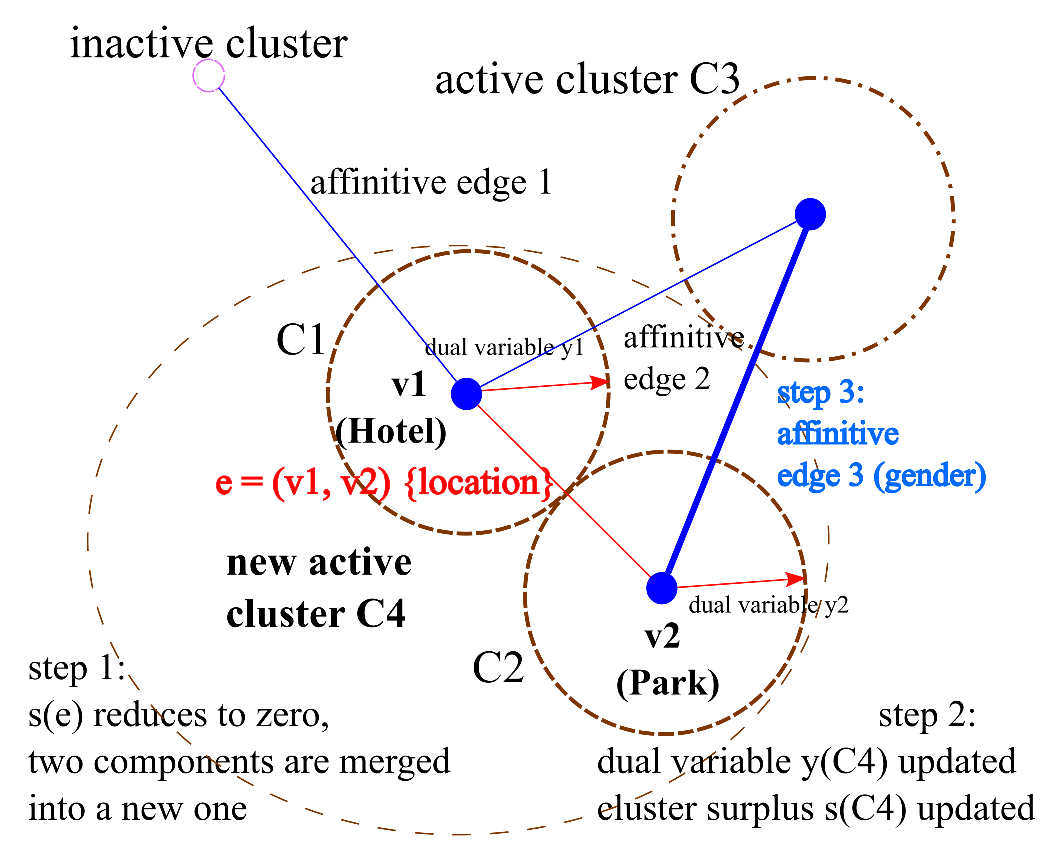
\includegraphics[scale=0.38]{./fig/runningExampleABD_v2.eps}}
\vspace{-1ex}
\caption{Dynamic clustering with affinitive edges}
\label{fig:backbonemerge}
\vspace{-3ex}
\end{figure}



\stitle{Time cost}.
It takes in total $O(|V|+|E|)$ time to initialize
the computation. In the growth phase (lines~2-9),
the total number of processed edges and connected clusters
is at most $(2^l-1)|E|$; and each processing
takes $O(\log|V|)$ time by accessing priority queues
$\Q_E$ and $\Q_P$. \merge and \refine take
$O(|V|)$ time. The total time cost
is thus
$O((2^l-1)|E|\log|V|)$. Putting these together, Theorem~\ref{theo-approx}
follows.








%%% problem definition

\vspace{-1ex}
%%%%%%%%%%%%%%%%%%% Section 8 %%%%%%%%%%%%%%%%%%%%%%%
\section{EM-based Heuristic}
\label{sec-em}

The fixed-parameter approximation is feasible when
the parameter
$l$ = $\max |\A(v)\cap\A(v')|$ ($v, v'\in V$) is small,
but can be expensive when $|\A|$ is large.
Moreover, the closeness function may not be available
for all the affinitive attributes. For example,
users may only specify interested affinitive attributes
but are not aware of a proper closeness measure for
the attributes. We next introduce
a faster heuristic algorithm that
can quickly infer the backbones without requiring
any closeness functions, and can quickly response
to new queries with changed interested nodes.

\stitle{Overview}. As no closeness functions are available for $\A$,
\ie no semantic closeness is known among attribute values,
the main idea is to dynamically infer the edge cost $C$
via an {\em edge generation model} $\M$, based on a practical assumption
that the likelihood of the existence of an edge $e$= $(v,v')$
is determined by the node attributes $\A(v)$ and $\A(v')$
and their values.
Our second algorithm, denoted as~\heuabd, performs a
once-for-all learning process to
compute an edge generation model $\M$, characterized by
an underlying stochastic
network generative model~\cite{kim2011modeling}.
Upon the specification of interested nodes $V_I$,
\heuabd dynamically infers a backbone $T$
with affinitive attributes and corresponding cost
$C(\cdot)$ from $\M$, such that the likelihood
of existence of $T$ is maximized.

\vspace{.5ex}
The algorithm ~\heuabd has two major components:
edge generation model learning, and
attribute inference.

\stitle{Learning edge generation model}.
We revise the multiplicative attribute graph model~\cite{kim2011modeling}
to an edge generation model with affinitive attributes,
which quantifies $C$ as:
\[
C(e, F_T(e), \M) = \prod^{|F_T(e)|}_{i=1}M_{A_i}[F_{A_i}(v)][F_{A_i}(v')]
\]
Here $M_i\in \M$ is an affinity matrix
associated to an attribute $A_i\in \A$.
For each attribute $A\in \A$ and matrix $M_A$,
the entry $M_A[j][k]\in [0,1]$ refers
to the probability
that an edge $(v,v')$ exists when
$F_A(v)$ (resp. $F_A(v')$) takes the $j$-th (resp. $k$-th) value
in $\adom(A)$.

\vspace{.5ex}
Algorithm~\heuabd invokes a procedure~\learn to
learn the affinity matrix $\M$.
Specifically, the probability
that $E$ exists given
node attribute values can be expressed
as
\[
\pr(E|\A, \M) = \prod_{(v,v')\in E}C(e, \A, \M)\prod_{(v,v')\not\in E}(1-C(e, \A, \M))
\]
The procedure \learn aims to identify
$\M$ by solving $\arg\max_{\M}\pr(E|\A,\M)$.
To this end, \learn applies a
maximum likelihood estimation (\kw{EM})
process to compute $\M$.
To reduce the learning cost, we
take a similar strategy as~\cite{kim2011modeling}
which considers that each attribute follows
Bernoulli distribution.

\stitle{Dynamic inference}.  The procedure~\learn
is a {\em once-for-all} process. Upon receiving nodes of interests $V_I$,
\heuabd invokes a second procedure~\infer,
which computes backbones by
incorporating the inference of affinitive
attributes to the process of clustering.

Procedure~\infer follows a similar clustering
process as in~\approxabd. It started by
initializing $\P$, and iteratively groups
clusters upon the verification of \isgrow and
\ismerge. The major difference is that it applies a
heuristic variant of the procedure~\updateAE,
without enumerating affinitive edges for each cluster.
More specifically,
given a cluster $P$, it first identifies
all the edges with one end node
in $P$. For each edge $e$=$(v,v')$, it
infers a set of affinitive attributes $F(e)$ directly,
by solving
\[ \argmax_{F(e)\subseteq\A(v)\cap\A(v')} C(e, F(e), \M)
\]
Given the independent likelihood of edges,
a heuristic is to sort and select top-k
attributes $A_i\in F(e)\subseteq\A(v)\cap\A(v')$
with the largest values
$M_{A_i}[F_{A_i}(v)][F_{A_i}(v')]$.
This can be inferred at run time,
whenever two clusters are merged.



%%%%%%%%%%%%%%%%%%%%%%%%%%%%%%%%%%%%%%%%
\begin{figure}[tb!]
\begin{center}
{\small
\begin{minipage}{3.36in}
\myhrule
\vspace{-1ex}
%%%%%%%%%%%%%%%%%Algorithm \paragfd%%%%%%%%%%%%
\mat{0ex}{
{\bf Algorithm}~\heuabd\\
\sstab {\sl Input:\/} \= graph $G$, interested nodes $V_I$.\\
{\sl Output:\/} an attribute-driven backbone $T$.\\
%%%%%%%%%%%%%
\bcc \hspace{3.6ex}\= \If cost model is not specified \Then \\
\icc\> \vspace{2ex} $\M$ := \learn(G, $\A$); \\
\icc\> $T$ := \infer(G, $\M$, $\A$, $V_I$); \\
\icc\> \Return $T$;
}
\vspace{-2ex}
\myhrule
\end{minipage}
}
\end{center}
\vspace{-2ex}
\caption{Algorithm~\heuabd} \label{fig:heuabd}
\vspace{-4ex}
\end{figure}


The algorithm~\heuabd is illustrated in
Fig.~\ref{fig:heuabd}.

\stitle{Performance analysis}.
It takes the procedure~\learn  $O(|A|^2|E|)$
time to learn the affinity matrix from scratch.
The time that infers the top-$k$ best affinitive
attributes for each cluster
is in $O(|A|\log|k|)$ time, and
in total $O(|A|\log|k||E|)$ for
all the edges. As the
affinitive attributes and the edge costs
are dynamically inferred,
it takes $O(|E|\log |V| + |V|)$ time for
\infer to simulate \GW scheme that
computes a prize-collecting Steiner tree.
It thus takes in total
$O(|A|^2|E| + |A|\log|k||E| + |E|\log |V| + |V|)$
time to compute backbones from scratch,
and $O(|A|\log|k||E| + |E|\log |V| + |V|)$
time given the matrix $\M$ which is learned once for all.





\vspace{-1ex}
%%%%%%%%%%%%%%%%%%% Section 8 %%%%%%%%%%%%%%%%%%%%%%%
\section{Online Approximate Optimal Backbones}
\label{sec-onliapprox}

\warn{The online approximate optimal backbones algorithm is put here.}
\vspace{-1ex}
%%%%%%%%%%%%%%%%%%% Section 8 %%%%%%%%%%%%%%%%%%%%%%%
\section{Online EM-Based Heuristic}
\label{sec-onliapprox}

\warn{The online EM-Based heuristic algorithm is put here.}
%\vspace{-1ex}
%%%%%%%%%%%%%%%%%%% Section 8 %%%%%%%%%%%%%%%%%%%%%%%
\section{Experiment}
\label{sec-expt}



\section {Conclusion}

We have introduced attributed backbones, 
which explicitly incorporate affinitive attributes 
to interpret connectivity in attributed networks. 
We have developed both approximation and 
fast heuristics, to cope with backbone detection 
in networks with small number of attributes, and 
with large attribute size and no explicitly specified 
edge cost model, respectively. 
Our experimental study verified that 
these algorithms can efficiently identify 
interpretable critical structures that 
cannot be identified by conventional 
community detection. 
A future work is to generalize 
our methods to identify 
attribute-driven graphs 
under constraints such as density. \warn{add more about online part.} 




% use section* for acknowledgment
%%%%%%%%%%%%%%%%%%%%%Comment this part%%%%%%%%%%%%%%%%%%
%%%%%%%%%%%%
%\ifCLASSOPTIONcompsoc
  % The Computer Society usually uses the plural form
  %\section*{Acknowledgments}
%\else
  % regular IEEE prefers the singular form
  %\section*{Acknowledgment}
%\fi
%%%%%%%%%%%%%%


\bibliographystyle{IEEEtran}
%\begin{small}
\bibliography{paper}







% that's all folks
\end{document}


